\documentclass[10pt]{beamer}
\usetheme{Rochester}

% load syscop style
\usepackage{style/syscop}

%--------------------------------------------------
%  TITLE
%--------------------------------------------------

\title[\texttt{acados}]{\huge \texttt{acados}}
\subtitle{\large A rapid prototyping tool for NMPC}
\author[R. Verschueren and M. Diehl]{Robin V, Dimitris K, Andrea Z, Rien Q, Niels v. D, Joris G, and Moritz Diehl}
\institute{Systems Control and Optimization laboratory}
\date[\today]{\today }


%--------------------------------------------------
% Useful packages
%--------------------------------------------------

\usepackage{mathtools}
\usepackage{graphicx}
\usepackage{wasysym}

\begin{document}

\InsertTitle

\begin{frame}{How things were until now}
	\begin{center}
		\Huge \texttt{www.acadotoolkit.org}
	\end{center}
	\vspace{0.5cm}
	
	Key Properties of ACADO Toolkit [Houska et al 2009]
	\begin{itemize}
		\item Open Source (LGPL)
		\item \textbf{A}utomatic \textbf{C}ontrol \textbf{A}nd 	\textbf{D}ynamic \textbf{O}ptimization
		\item User friendly interface close to mathematical syntax
	\end{itemize}
	
	\pause
	
	Multiplatform support
	\begin{itemize}
		\item C++: Linux, OS X, Windows
		\item MATLAB
	\end{itemize}	
\end{frame}


\begin{frame}{ACADO developers (past and current)}
	\begin{center}
		\includegraphics[scale=0.57]{dev.eps}
	\end{center}
\end{frame}

\begin{frame}{ACADO Code Generation Toolkit}
	\begin{columns}
		\begin{column}{0.5\textwidth}
			Pro
			\begin{itemize}
				\item<1-> Easy to use, 
				\item<2-> Fast NMPC/MHE solvers,
				\item<3-> Interfaced to external solvers,
				\item<4-> Comes with own AD,
			\end{itemize}
		\end{column}
		\begin{column}{0.6\textwidth}
			Con
			\begin{itemize}
				\item<1-> ... but codebase difficult to maintain
				\item<2-> ... but with a lot of global data
				\item<3-> ... but hard coupling with new ones
				\item<4-> ... but not compatible with CasADi
			\end{itemize}
		\end{column}	
	\end{columns}
\end{frame}

\begin{frame}{Code generation}
	\begin{figure}
		\centering
		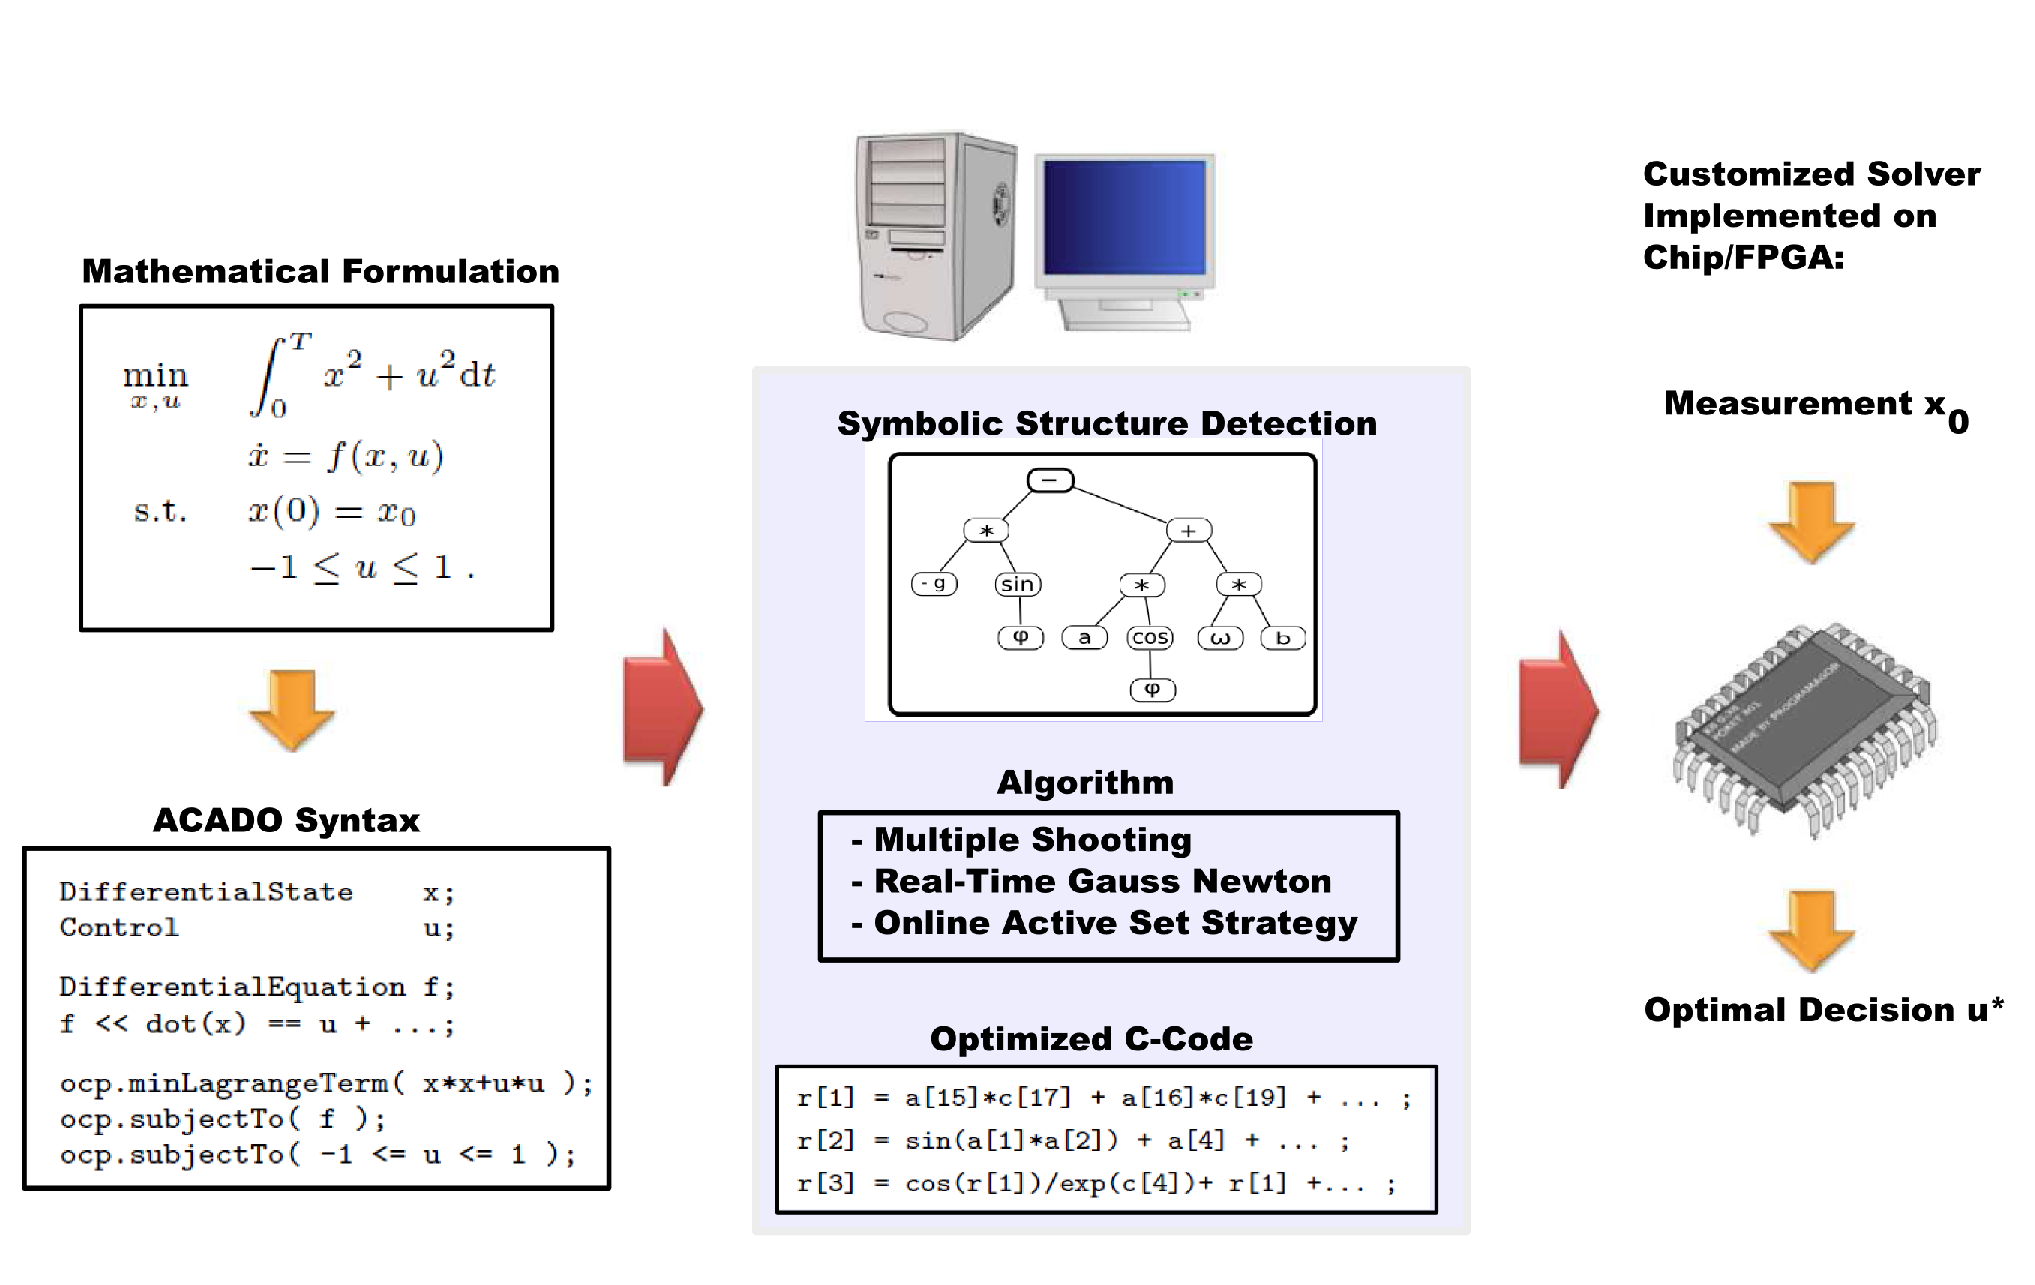
\includegraphics[width=0.8\linewidth]{AcadoCodeGen}
		\label{fig:acadocodegen}
	\end{figure}
	\pause
	\centering \huge \fbox{But is codegen really necessary?}
\end{frame}

\begin{frame}{Code generation}
	Why code generation?
	\begin{itemize}
		\item eliminate computations 
		\item known dimensions and sparsity patterns 
		\item no dynamic memory
		\item code reorganization, $\ldots$
	\end{itemize}
	\pause
	But code generation
	\begin{itemize}
		\item increases code size
		\item creates unreadable code
		\item only really makes sense at the bottleneck $\rightarrow$ linear algebra
	\end{itemize}
\end{frame}

\begin{frame}{A different idea}
	Instead of code-generated code, we want
	\begin{itemize}
		\item maintainable, 
		\item extensible,
		\item fast code,
		\item with efficient linear algebra kernels,
		\item available from \textsc{MATLAB} and Python.
	\end{itemize}
	\centering \huge $\rightarrow$ \texttt{acados}
\end{frame}

\begin{frame}{Interfaces}
	The structure of \texttt{acados} is based on internal interfaces:
	\begin{itemize}
		\item OCP QP interface,
		\item condensing interface,
		\item integrator interface,
		\item AD interface,
		\item Hessian regularization interface,
		\item \ldots
	\end{itemize}
	If a solver sticks to a certain interface, it can be swapped quickly for another one \\ \centering $\rightarrow$ Rapid Prototyping
\end{frame}

\begin{frame}{Status}
	As of now: one NMPC example in \texttt{C99} with
	\begin{itemize}
		\item Model: [Chen\&Allgoewer 1998]
		\item Integrator: Runge-Kutta 4
		\item Condensing: $N^2$
		\item QP solver: \texttt{qpOASES3.0}
	\end{itemize}
	\pause
	\begin{alertblock}{}
		\centering $0.63\,\mathrm{ms}$ per iteration, \\ only 2x slower than ACADO code generated code, \\ not bad for first 'plain vanilla' attempt \smiley
	\end{alertblock}
\end{frame}

\begin{frame}{Codebase}
	Located at 
	\centering \large \texttt{https://github.com/acados/acados}
	\vspace{0.5cm}
	\normalsize
	\begin{itemize}
		\item Completely written in \texttt{C99}
		\item Each interface has its own header file
		\item Data passed around by pointers to \texttt{struct}s
	\end{itemize}
	\pause
	\flushleft TODO:
	\begin{itemize}
		\item Interface with CasADi (and thus \textsc{MATLAB}/Python)
		\item Use BlasFEO's (former HPMPC) highly optimized linear algebra
		\item Implement many more new solvers
		\item Real-life examples
		\item \ldots
	\end{itemize}
\end{frame}

\bibliographystyle{plain}

\end{document}
